\documentclass{article}
\usepackage{graphicx}
\usepackage{amssymb}
\usepackage{amsmath}
\usepackage[backend=bibtex,style=ieee,bibencoding=ascii,sorting=none]{biblatex}
\usepackage{fancyhdr}
\usepackage{geometry}

\geometry{left=1in, right=1in, top=1in}
\pagestyle{fancy}
\fancyhf{}
\fancyhead[L]{Carlos Martinez-Villar}
\fancyhead[R]{STAT9100--Statistical Learning with Networks, Final Project Report}

\title{Final Project Report\\STAT 9100 - Statistical Learning with Networks}
\author{Carlos Martinez-Villar}
\date{\today}

\addbibresource{refs}

\begin{document}
%	\maketitle
	
	%%%%%%%%%%%%%%%%%%%%%%%%%%%%%%
	% INTRODUCTION
	%%%%%%%%%%%%%%%%%%%%%%%%%%%%%%
	\section{Introduction}
	The present report includes an attempt at fulfilling the requirements for the course's final project by discussing Hopfield networks and their properties in relation to the subjects presented throughout this semester. 
	The report is organized as follows: the second section includes a somewhat detailed description of the Hopfield model. Subsections describe the equations and rules that were needed to implement and use a simple working version. The last two of these subsections include a broader discussion of this type of model with analogies to statistical physics and the Ising model. The third section includes results that showed the model was correctly implemented and a brief discussion of the shortcomings in this implementation. 
	
	%%%%%%%%%%%%%%%%%%%%%%%%%%%%%%
	% MODEL
	%%%%%%%%%%%%%%%%%%%%%%%%%%%%%%	
	\section{Hopfield's Model and Methods}
	
	The bulk of the method used here was established early on–in the original work–by Hopfield in \cite{hopfield1982neural}  and \cite{hopfield1984neurons}. Given that, the more recent variations of these models have focused on tweaking the original models to either generalize over new types of data or increase their memory capacity. These recent extensions, like those by Krotov and Hopfield \cite{krotov2016dense}, have yieded more expressive models that are beyond the scope of this report. It is important to note, however, that these latter approaches have brought with them a resurgence to Hopfield networks in the sense that these have become once again relevant. \\
	\cite{hebb2005organization}
	\cite{mackay2003information}
	
	\subsection{Node Update Rule}
	
	We can set the value of a node $j$ in the network by using the update rule 
	\begin{equation}\label{nodeupdate}
	x_j = \begin{cases}
		 1  & \text{if } \sum^{}_{i \neq j} x_i W_{ij}  < -b_j \\
		-1  & \text{if } \sum^{}_{i \neq j} x_i W_{ij} \ge -b_j
	\end{cases}
	\end{equation}
	
	\subsection{Setting W: Updating Edge Weights Between Nodes}
	
	
	\subsubsection{Storing a Pattern in the Network}
	
	If we have a pattern we would like the network to recall, we can set the weights (edges) 
	
	\subsubsection{Storing Multiple Patterns}	
	
	\subsection{The Idea of Energy in Hopfield Networks}
	\begin{equation}
		E = - \sum^{}_{i \neq j} s_i s_j w_{ij} - \sum^{}_{i} s_i b_i
	\end{equation}		
	
	\begin{equation}
		E = -\mathbf{s}^T W\mathbf{s} - \mathbf{s}^T b	
	\end{equation}
	
	\subsubsection{Relation to Gradient Descent}
	Gradient descent is today the most common method for 
	
	This derivative of $\frac{d x_j}{dt}$ agrees with the update rule equation prescribed iby \ref{nodeupdate}.
	
	\subsubsection{Settling to an Energy Minimum}
	
	
	%%%%%%%%%%%%%%%%%%%%%%%%%%%%%%
	% EXPs
	%%%%%%%%%%%%%%%%%%%%%%%%%%%%%%		
	\section{Experiments (with a Discrete System)}

	Similarly, we can set up vectors of length 16 to be orthogonal in the following way
	
	\begin{center}
	\texttt{[\ 1,\ 1,\ 1,\ 1,\ 1,\ 1,\ 1,\ 1,-1,-1,-1,-1,-1,-1,-1,-1]}\\
	\texttt{[\ 1,\ 1,\ 1,\ 1,-1,-1,-1,-1,\ 1,\ 1,\ 1,\ 1,-1,-1,-1,-1]}\\
	\texttt{[\ 1,\ 1,-1,-1,\ 1,\ 1,-1,-1,\ 1,\ 1,-1,-1,\ 1,\ 1,-1,-1]}
	\end{center}


	
	\subsection{Computing a Probability Distribution}
	\subsubsection{Exhaustive computation}
	
	
	\section{Graded Response}
	As shown in \cite{hopfield1984neurons}
	\subsubsection{Metropolis-Hastings}	
	
		

	\section{Conclusions and possible research prospects}
	Taken alone, the model introduced by Hopfield can be seen to have two shortcomings that make it seem irrelevant.


	%%%%%%%%%%%%%%%%%%%%%%%%%%%%%%
	% REFS
	%%%%%%%%%%%%%%%%%%%%%%%%%%%%%%	
	\pagebreak
	\printbibliography[title={References}]
	
	%%%%%%%%%%%%%%%%%%%%%%%%%%%%%%
	% FIGURES, TABLES, ETC.
	%%%%%%%%%%%%%%%%%%%%%%%%%%%%%%	
	\pagebreak
	\section*{Appendix of Figures}
	
	\begin{center}
%	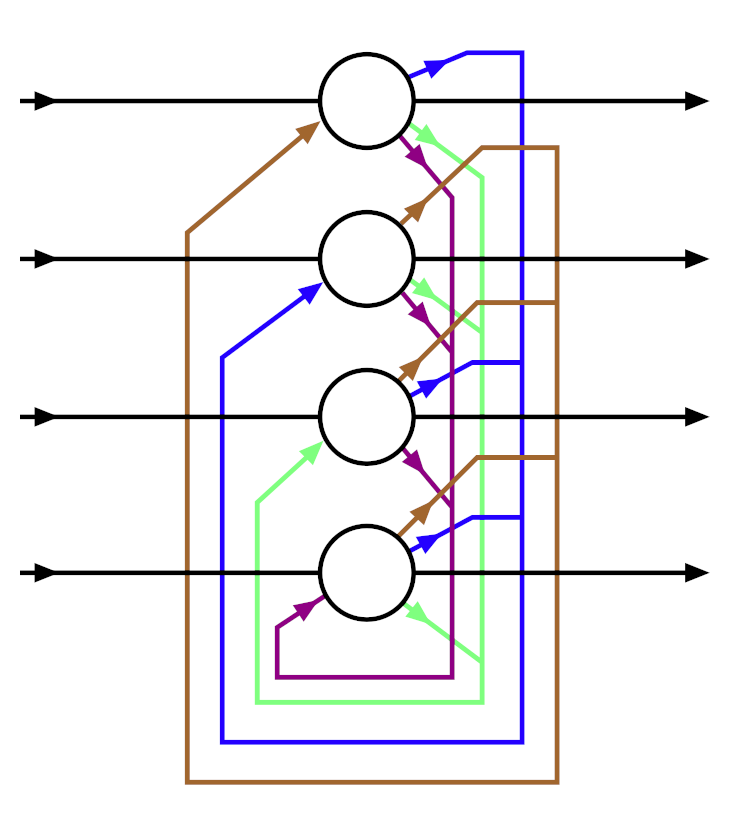
\includegraphics[width=0.3\textwidth]{../img/hopfieldnet.png}	
	\end{center}
	
	\begin{center}
	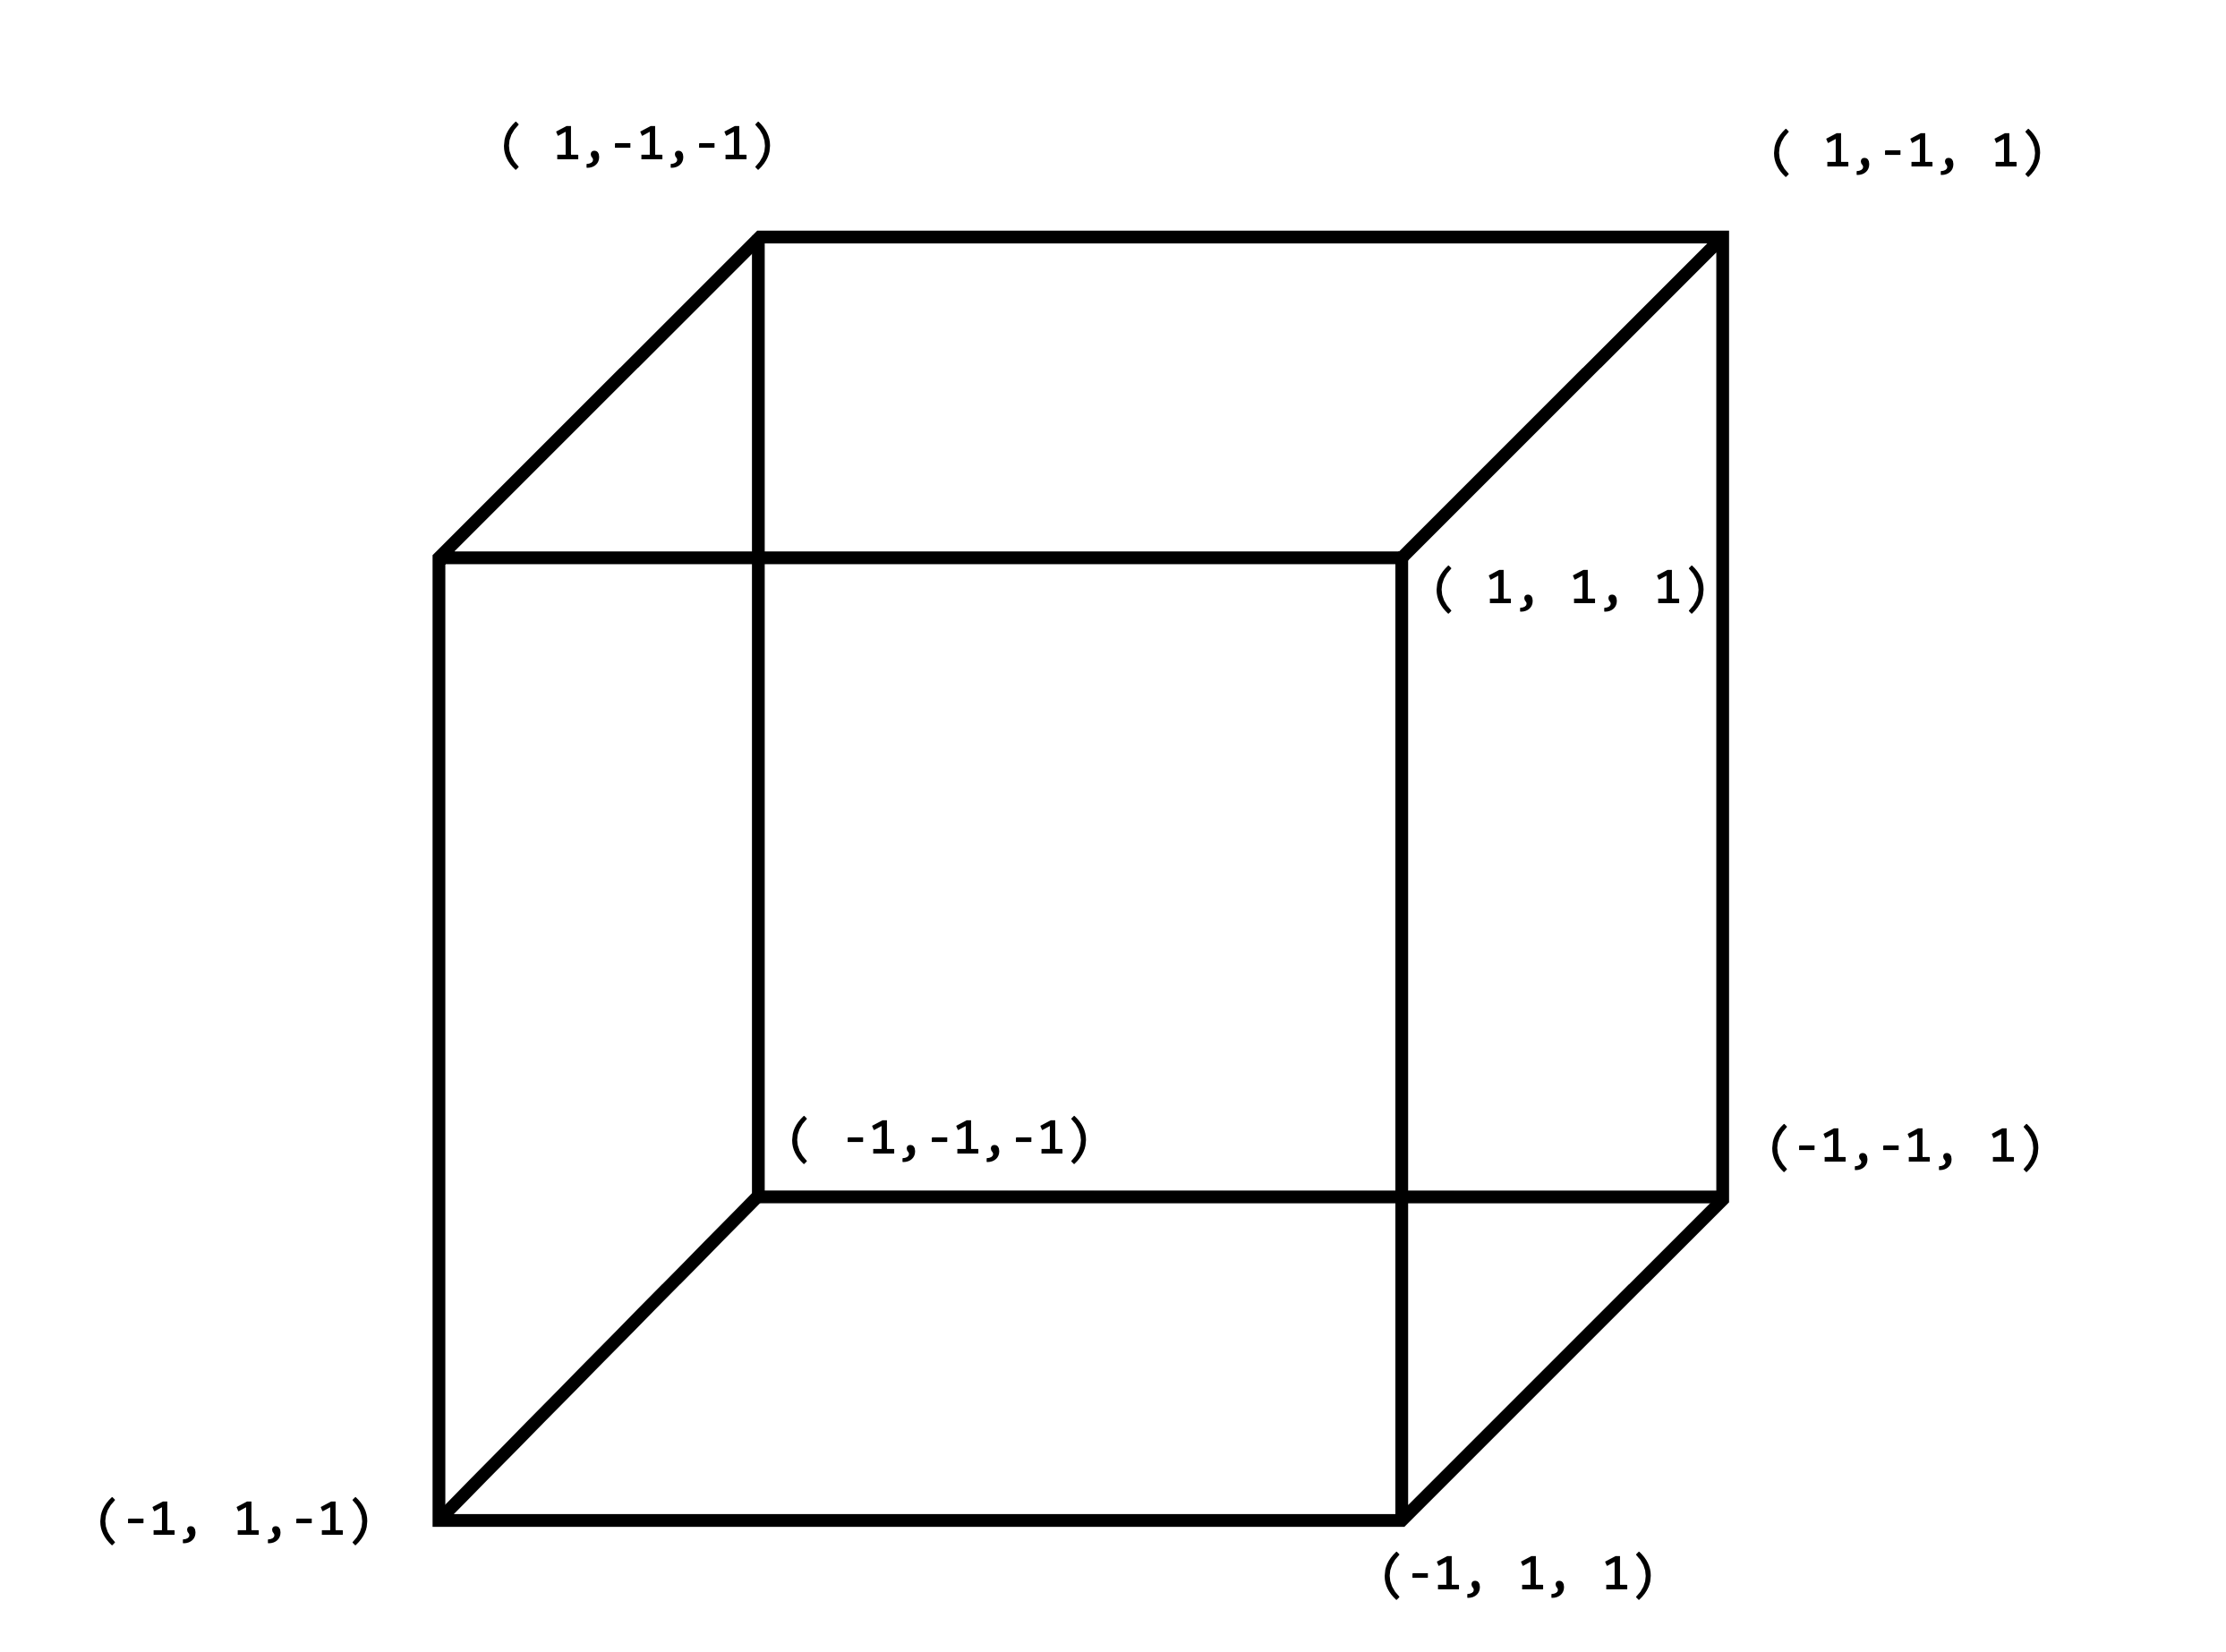
\includegraphics[width=0.5\textwidth]{../img/hypercube.png}
	\end{center}		
	
	
	\begin{center}
	
\includegraphics[scale=0.5]{../img/small_letters.png}	
	\end{center}
	\begin{center}
	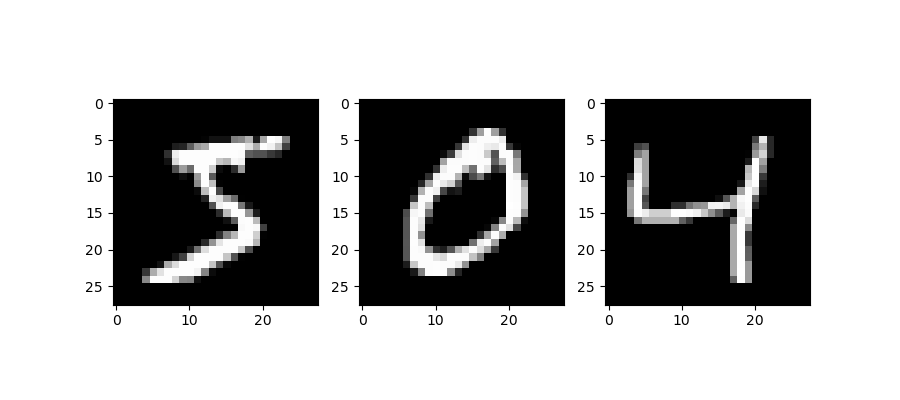
\includegraphics[scale=0.5]{../img/digits.png}	
	\end{center}	

	\begin{center}
	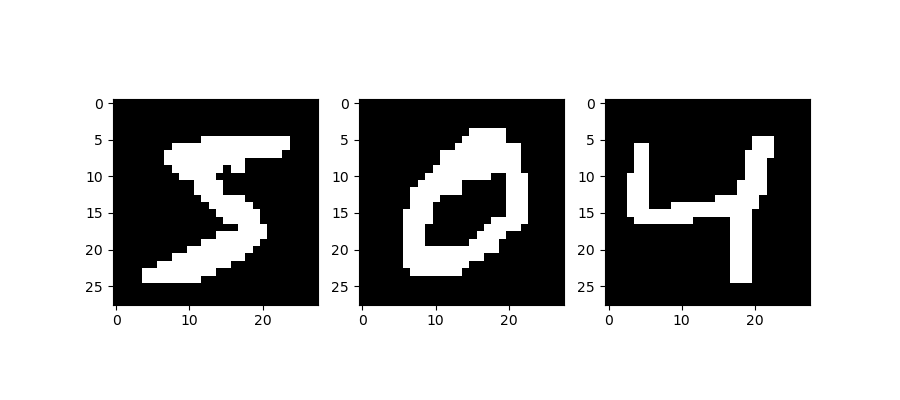
\includegraphics[scale=0.5]{../img/digits_shifted.png}	
	\end{center}	
	
	\begin{center}
	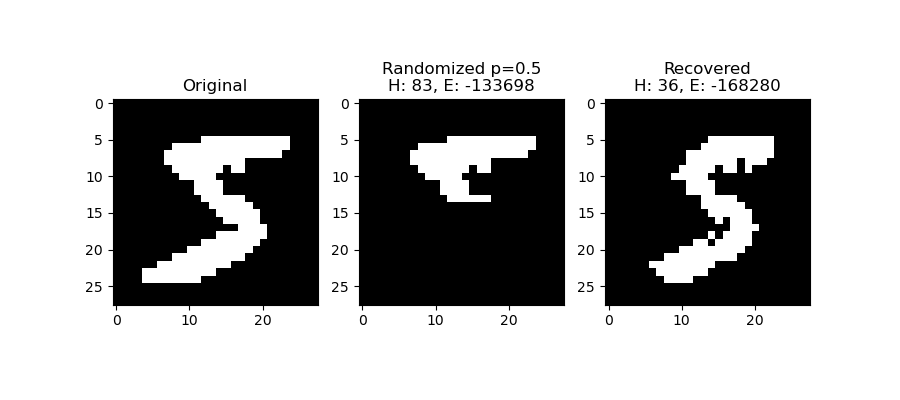
\includegraphics[scale=0.5]{../img/digits_result_good_covered.png}	
	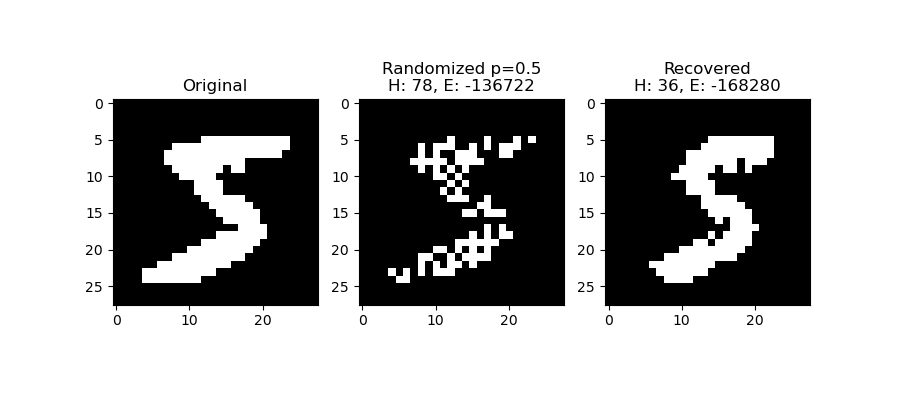
\includegraphics[scale=0.5]{../img/digits_result_good_random.png}	
	\end{center}	
	
\end{document}
